\documentclass[a4paper, titlepage]{article}
\usepackage{cite}
\usepackage{listings}
\usepackage{graphicx}

\begin{document}
\title{
Heriot Watt University \protect\\ Rigorous Methods for Software Engineering\protect\\A High Integrity Software Development Exercise
}

\author{Vytautas Tumas}

\maketitle
\tableofcontents
\section{Introduction}
The aim of the coursework was to produce a software based Automatic Vessel Protection (AVP) system using the SPARK approach to high integrity Ada. The task was to develop the system-critical control component as well as the implementation details of the boundary packages.
\section{Assumptions}
Here is a list of assumptions made during the development of the system:
\begin{itemize}
\item Because this is an embedded system, I've assumed that Sensor count will not exceed 3, thus I used three variables to store their value instead of an array.
\item I've assumed that once the escape valve is enabled, it can only be disabled if the reset mechanism is enabled.
\end{itemize}
\section{Class Diagram}
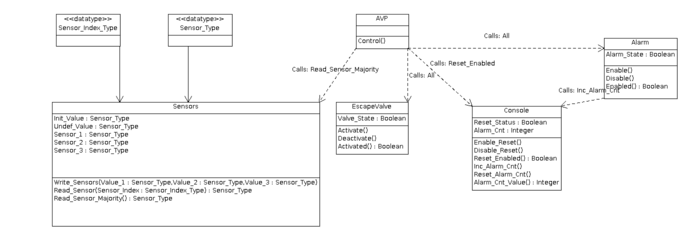
\includegraphics[scale=0.5]{diagram}
\section{Listing files}
\subsection{Alarm}
\subsubsection{Specification}
{\tiny
\begin{lstlisting}
           *******************************************************
                            Listing of SPARK Text
                              Examiner GPL 2012
             Copyright (C) 2012 Altran Praxis Limited, Bath, U.K.
           *******************************************************


                        DATE : 21-OCT-2015 10:44:13.36

Line
   1  --# inherit Console;
   2  package Alarm
   3     --# own State;
   4     --# initializes State;
   5  is
   6     procedure Enable;
   7     --# global in out Console.Alarm_Cnt;
   8     --#  out State;
   9     --# derives State from & Console.Alarm_Cnt from Console.Alarm_Cnt;
  10  
  11  
  12     procedure Disable;
  13     --# global out State;
  14     --# derives State from ;
  15  
  16     function Enabled return Boolean;
  17     --# global in State;
  18  
  19  end Alarm;
  20  
  21  

Note: Flow analysis mode is automatic

--End of file--------------------------------------------------
\end{lstlisting}
}
\subsubsection{Body}
{\tiny
\begin{lstlisting}
           *******************************************************
                            Listing of SPARK Text
                              Examiner GPL 2012
             Copyright (C) 2012 Altran Praxis Limited, Bath, U.K.
           *******************************************************


                        DATE : 21-OCT-2015 10:47:37.70

Line
   1  with Console;
   2  package body Alarm 
   3  is
   4      State: Boolean;
   5      procedure Enable
   6      is
   7      begin
   8          Console.Inc_Alarm_Cnt;
   9          State := True;
  10      end Enable;

+++        Flow analysis of subprogram Enable performed 
           (information-flow mode): no errors found.

  11  
  12      procedure Disable
  13      is
  14      begin
  15          State := False;
  16      end Disable;

+++        Flow analysis of subprogram Disable performed 
           (information-flow mode): no errors found.

  17  
  18  
  19      function Enabled return Boolean
  20      is
  21      begin
  22          return State;
  23      end Enabled;

+++        Flow analysis of subprogram Enabled performed 
           (information-flow mode): no errors found.

  24  
  25  begin
  26      -- init
  27      State := False;
  28  end Alarm;

+++        Flow analysis of package initialization 
           performed: no errors found.


Note: Flow analysis mode is automatic


--End of file--------------------------------------------------

\end{lstlisting}
}
\subsection{Console}
\subsubsection{Specification}
{\tiny
\begin{lstlisting}
           *******************************************************
                            Listing of SPARK Text
                              Examiner GPL 2012
             Copyright (C) 2012 Altran Praxis Limited, Bath, U.K.
           *******************************************************


                        DATE : 21-OCT-2015 10:44:13.36

Line
   1  package  Console
   2    --# own Reset_Status, Alarm_Cnt;
   3    --# initializes Reset_Status, Alarm_Cnt;
   4  is
   5      Reset_Status: Boolean;
   6      Alarm_Cnt: Integer;
   7     
   8     procedure Enable_Reset;
   9        --# global out Reset_Status;
  10        --# derives Reset_Status from ; 
  11     
  12     procedure Disable_Reset;
  13       --# global out Reset_Status;
  14       --# derives Reset_Status from ;  
  15     
  16     function Reset_Enabled return Boolean;
  17       --# global in Reset_Status;  
  18     
  19     procedure Inc_Alarm_Cnt;
  20       --# global in out Alarm_Cnt;
  21       --# derives Alarm_Cnt from Alarm_Cnt;
  22  
  23     procedure Reset_Alarm_Cnt;
  24        --# global out Alarm_Cnt;
  25        --# derives Alarm_Cnt from ;
  26     
  27     function Alarm_Cnt_Value return Integer;
  28     --# global in Alarm_Cnt;
  29  
  30  end Console;

Note: Flow analysis mode is automatic


--End of file--------------------------------------------------

\end{lstlisting}
}
\subsubsection{Body}
{\tiny
\begin{lstlisting}
           *******************************************************
                            Listing of SPARK Text
                              Examiner GPL 2012
             Copyright (C) 2012 Altran Praxis Limited, Bath, U.K.
           *******************************************************


                        DATE : 21-OCT-2015 10:47:37.68

Line
   1  package  body Console is   
   2     procedure Enable_Reset 
   3     is
   4     begin
   5          Reset_Status := True;
   6     end Enable_Reset;

+++        Flow analysis of subprogram Enable_Reset 
           performed (information-flow mode): no errors found.

   7  
   8     procedure Disable_Reset 
   9     is
  10     begin
  11          Reset_Status := False;
  12     end Disable_Reset;

+++        Flow analysis of subprogram Disable_Reset 
           performed (information-flow mode): no errors found.

  13  
  14     function Reset_Enabled return Boolean
  15     is
  16     begin
  17          return Reset_Status;
  18     end Reset_Enabled;

+++        Flow analysis of subprogram Reset_Enabled 
           performed (information-flow mode): no errors found.

  19     
  20     procedure Inc_Alarm_Cnt
  21     is
  22     begin
  23        -- prevent overflow
  24        if Alarm_Cnt < Integer'Last then
  25          Alarm_Cnt := Alarm_Cnt + 1;
  26        end if;
  27     end Inc_Alarm_Cnt;

+++        Flow analysis of subprogram Inc_Alarm_Cnt 
           performed (information-flow mode): no errors found.

  28     
  29     procedure Reset_Alarm_Cnt
  30     is
  31     begin
  32          Alarm_Cnt := 0;
  33     end Reset_Alarm_Cnt;

+++        Flow analysis of subprogram Reset_Alarm_Cnt 
           performed (information-flow mode): no errors found.

  34        
  35     function Alarm_Cnt_Value return Integer
  36     is
  37     begin
  38          return Alarm_Cnt;
  39     end Alarm_Cnt_Value;

+++        Flow analysis of subprogram Alarm_Cnt_Value 
           performed (information-flow mode): no errors found.

  40  begin
  41      -- init
  42      Reset_Status := False;
  43      Alarm_Cnt := 0;
  44  end Console;

+++        Flow analysis of package initialization 
           performed: no errors found.

  45  
  46  

Note: Flow analysis mode is automatic


--End of file--------------------------------------------------
\end{lstlisting}
}
\subsection{Sensors}
\subsubsection{Specification}
{\tiny
\begin{lstlisting}
           *******************************************************
                            Listing of SPARK Text
                              Examiner GPL 2012
             Copyright (C) 2012 Altran Praxis Limited, Bath, U.K.
           *******************************************************


                        DATE : 20-OCT-2015 10:55:16.81

Line
   1  package Sensors
   2     --# own State;
   3     --# initializes State;
   4  is
   5     Init_Value:  constant := 0;
   6     Undef_Value: constant := 200; -- range of valid pressure readings is 0..199. A value of 200 denotes an undefined reading.
   7  
   8     subtype Sensor_Type is Integer range 0..200;
   9     subtype Sensor_Index_Type is Integer range 1..3;
  10           
  11     procedure Write_Sensors(Value_1, Value_2, Value_3: in Sensor_Type);
  12     --# global out State;
  13     --# derives State from Value_1, Value_2, Value_3;
  14  
  15     function Read_Sensor(Sensor_Index: in Sensor_Index_Type) return Sensor_Type;
  16     --# global in State;
  17  
  18     function Read_Sensor_Majority return Sensor_Type;
  19     --# global in State;
  20     
  21  end Sensors;

Note: Flow analysis mode is automatic


--End of file--------------------------------------------------

\end{lstlisting}
}
\subsubsection{Body}
{\tiny
\begin{lstlisting}
           *******************************************************
                            Listing of SPARK Text
                              Examiner GPL 2012
             Copyright (C) 2012 Altran Praxis Limited, Bath, U.K.
           *******************************************************


                        DATE : 21-OCT-2015 10:51:46.13

Line
   1  package body Sensors
   2     --# own State is Sensor_1, Sensor_2, Sensor_3;
   3  is
   4  
   5     -- initializing at 0 might be bad
   6     Sensor_1: Sensor_Type;
   7     Sensor_2: Sensor_Type;
   8     Sensor_3: Sensor_Type;
   9  
  10     procedure Write_Sensors(Value_1, Value_2, Value_3: in Sensor_Type) 
  11     --# global out Sensor_1, Sensor_2, Sensor_3;
  12     --# derives Sensor_1 from Value_1 & Sensor_2 from Value_2 & Sensor_3 from Value_3;
  13     is
  14     begin
  15        Sensor_1 := Value_1;
  16        Sensor_2 := Value_2;
  17        Sensor_3 := Value_3;
  18     end Write_Sensors;

+++        Flow analysis of subprogram Write_Sensors 
           performed (information-flow mode): no errors found.

  19  
  20     function Read_Sensor(Sensor_Index: in Sensor_Index_Type) return Sensor_Type
  21     --# global in Sensor_1, Sensor_2, Sensor_3;
  22     is
  23        t : Sensor_Type := Init_Value;
  24     begin
  25        if Sensor_Index < Sensor_Index_Type'Last then
  26           if Sensor_Index = 1 then
  27              t := Sensor_1;
  28           elsif Sensor_Index = 2 then
  29              t := Sensor_2;
  30           else
  31              t := Sensor_3;
  32           end if;
  33        end if;
  34        return t;
  35     end Read_Sensor;

+++        Flow analysis of subprogram Read_Sensor 
           performed (information-flow mode): no errors found.

  36  
  37  
  38     function Read_Sensor_Majority return Sensor_Type 
  39     --# global in Sensor_1, Sensor_2, Sensor_3;
  40     is
  41        t: Sensor_Type;
  42     begin
  43     if Sensor_1 = Sensor_2 then
  44        t := Sensor_1;
  45     elsif Sensor_1 = Sensor_3 then
  46        t := Sensor_1;
  47     elsif Sensor_2 = Sensor_3 then
  48        t := Sensor_2;
  49     else
  50        t := Undef_Value;
  51     end if;
  52  
  53     return t;
  54     end Read_Sensor_Majority;

+++        Flow analysis of subprogram Read_Sensor_Majority 
           performed (information-flow mode): no errors found.

  55  begin
  56     Sensor_1 := Init_Value;
  57     Sensor_2 := Init_Value;
  58     Sensor_3 := Init_Value;   
  59  end Sensors;

+++        Flow analysis of package initialization 
           performed: no errors found.


Note: Flow analysis mode is automatic


--End of file--------------------------------------------------


\end{lstlisting}
}
\subsection{EscapeValve}
\subsubsection{Specification}
{\tiny
\begin{lstlisting}
           *******************************************************
                            Listing of SPARK Text
                              Examiner GPL 2012
             Copyright (C) 2012 Altran Praxis Limited, Bath, U.K.
           *******************************************************

                        DATE : 20-OCT-2015 10:56:17.25

Line
   1  package EscapeValve
   2     --# own State;
   3     --# initializes State;
   4  is
   5     procedure Activate;
   6     --# global out State;
   7     --# derives State from ;
   8  
   9     procedure Deactivate;
  10     --# global out State;
  11     --# derives State from ;
  12  
  13     function Activated return Boolean;
  14     --# global in State;
  15  
  16  end EscapeValve;
  17  
  18  

Note: Flow analysis mode is automatic

--End of file--------------------------------------------------
\end{lstlisting}
}
\subsubsection{Body}
{\tiny
\begin{lstlisting}
           *******************************************************
                            Listing of SPARK Text
                              Examiner GPL 2012
             Copyright (C) 2012 Altran Praxis Limited, Bath, U.K.
           *******************************************************


                        DATE : 20-OCT-2015 10:56:38.14

Line
   1  package body EscapeValve
   2     --# own State is Valve_State;
   3  is
   4     Valve_State: Boolean;
   5  
   6     procedure Activate
   7     --# global out Valve_State;
   8     --# derives Valve_State from ;
   9     is
  10     begin
  11        Valve_State := True;
  12     end Activate;

+++        Flow analysis of subprogram Activate performed 
           (information-flow mode): no errors found.

  13  
  14     procedure Deactivate
  15     --# global out Valve_State;
  16     --# derives Valve_State from ;
  17     is
  18     begin
  19        Valve_State := False;
  20     end Deactivate;

+++        Flow analysis of subprogram Deactivate performed 
           (information-flow mode): no errors found.

  21  
  22     function Activated return Boolean
  23     --# global in Valve_State;
  24     is
  25     begin
  26        return Valve_State;
  27     end Activated;

+++        Flow analysis of subprogram Activated performed 
           (information-flow mode): no errors found.

  28  
  29  begin
  30     Valve_State := False;
  31  end EscapeValve;

+++        Flow analysis of package initialization 
           performed: no errors found.

  32  
  33  

Note: Flow analysis mode is automatic


--End of file--------------------------------------------------

\end{lstlisting}
}
\subsection{AVP}
\subsubsection{Specification}
{\small
\begin{lstlisting}
           *******************************************************
                            Listing of SPARK Text
                              Examiner GPL 2012
             Copyright (C) 2012 Altran Praxis Limited, Bath, U.K.
           *******************************************************


                        DATE : 21-OCT-2015 10:44:13.37

Line
   1  --# inherit Sensors, Console, Alarm, EscapeValve;
   2  package AVP
   3  is
   4           
   5     procedure Control;
   6     --# global in Sensors.State, Console.Reset_Status;
   7     --#        in out Alarm.State, EscapeValve.State, Console.Alarm_Cnt;
   8  
   9     
  10  end AVP;

Note: Flow analysis mode is automatic


--End of file--------------------------------------------------

\end{lstlisting}
}
\subsubsection{Body}
{\small
\begin{lstlisting}
           *******************************************************
                            Listing of SPARK Text
                              Examiner GPL 2012
             Copyright (C) 2012 Altran Praxis Limited, Bath, U.K.
           *******************************************************


                        DATE : 21-OCT-2015 10:51:46.14

Line
   1  with Sensors, Console, Alarm, EscapeValve;
   2  package body AVP
   3  is
   4     procedure Control is
   5          Sensor_Value: Sensors.Sensor_Type;
   6     begin 
   7  
   8          Sensor_Value := Sensors.Read_Sensor_Majority;
   9     
  10          if EscapeValve.Activated = False then
  11  
  12              -- if normal
  13              if (Sensor_Value < 100) then
  14                  
  15                  -- if alarm is active
  16                  if Alarm.Enabled = True then
  17                      Alarm.Disable;
  18                  end if;
  19              elsif (Sensor_Value >= 100) then
  20                  -- check if value got reduced
  21                  -- if high
  22                  if(Sensor_Value <= 149) then
  23                      -- enable alarm
  24                      if Alarm.Enabled = False then
  25                          Alarm.Enable;
  26  
  27                      else -- if the alarm has already been activated activate the valve  
  28                              EscapeValve.Activate;
  29                      end if;
  30                  -- if critical
  31                  elsif (Sensor_Value >= 150) then
  32                      -- activate escape valve
  33                      EscapeValve.Activate;
  34                      -- if alarm not active - activate
  35                      if Alarm.Enabled = False then
  36                          Alarm.Enable;
  37                      end if;
  38                  end if;
  39              end if;
  40          end if;
  41          
  42          -- if reset mechanism is enabled
  43          if Console.Reset_Enabled = True then
  44              Alarm.Disable;
  45              EscapeValve.Deactivate;
  46          end if;
  47  
  48     end Control;

+++        Flow analysis of subprogram Control performed 
           (data-flow mode): no errors found.

  49     
  50  end AVP;

Note: Flow analysis mode is automatic


--End of file--------------------------------------------------

\end{lstlisting}
}
\section{Report}
{\tiny
\begin{lstlisting}
           *******************************************************
                         Report of SPARK Examination
                              Examiner GPL 2012
             Copyright (C) 2012 Altran Praxis Limited, Bath, U.K.
           *******************************************************


                        DATE : 21-OCT-2015 10:51:46.14

Options:
    noswitch
    noindex_file
    nowarning_file
    notarget_compiler_data
    config_file=gnat.cfg
    source_extension=ada
    listing_extension=lst
    nodictionary_file
    report_file=spark.rep
    nohtml
    vcg
    nostatistics
    fdl_identifiers=accept
    flow_analysis=auto
    language=95
    profile=sequential
    annotation_character=#
    rules=lazy
    error_explanations=off
    justification_option=full
    output_directory=report
    output_directory (actual)=/home/tapanito/university/rigsys/cw1/code/report/

Selected files:
   @AVP.smf


No Index files were used


Meta File(s) used were:
   AVP.smf
      /home/tapanito/university/rigsys/cw1/code/console.ads
      /home/tapanito/university/rigsys/cw1/code/console.adb
      /home/tapanito/university/rigsys/cw1/code/sensors.ads
      /home/tapanito/university/rigsys/cw1/code/sensors.adb
      /home/tapanito/university/rigsys/cw1/code/alarm.ads
      /home/tapanito/university/rigsys/cw1/code/alarm.adb
      /home/tapanito/university/rigsys/cw1/code/escapevalve.ads
      /home/tapanito/university/rigsys/cw1/code/escapevalve.adb
      /home/tapanito/university/rigsys/cw1/code/avp.ads
      /home/tapanito/university/rigsys/cw1/code/avp.adb


Full warning reporting selected


Target configuration file:
Line
   1  package Standard is
   2     type Integer is range -2**31 .. 2**31-1;
   3  end Standard;


Source Filename(s) used were:
   /home/tapanito/university/rigsys/cw1/code/console.ads
   /home/tapanito/university/rigsys/cw1/code/console.adb
   /home/tapanito/university/rigsys/cw1/code/sensors.ads
   /home/tapanito/university/rigsys/cw1/code/sensors.adb
   /home/tapanito/university/rigsys/cw1/code/alarm.ads
   /home/tapanito/university/rigsys/cw1/code/alarm.adb
   /home/tapanito/university/rigsys/cw1/code/escapevalve.ads
   /home/tapanito/university/rigsys/cw1/code/escapevalve.adb
   /home/tapanito/university/rigsys/cw1/code/avp.ads
   /home/tapanito/university/rigsys/cw1/code/avp.adb



Source Filename:   /home/tapanito/university/rigsys/cw1/code/console.ads
Listing Filename:  /home/tapanito/university/rigsys/cw1/code/report/console.lst

   Unit name:  Console
   Unit type:  package specification
   Unit has been analysed, any errors are listed below.

No errors found


Source Filename:   /home/tapanito/university/rigsys/cw1/code/console.adb
Listing Filename:  /home/tapanito/university/rigsys/cw1/code/report/console.lst

   Unit name:  Console
   Unit type:  package body
   Unit has been analysed, any errors are listed below.

No errors found


Source Filename:   /home/tapanito/university/rigsys/cw1/code/sensors.ads
Listing Filename:  /home/tapanito/university/rigsys/cw1/code/report/sensors.lst

   Unit name:  Sensors
   Unit type:  package specification
   Unit has been analysed, any errors are listed below.

No errors found


Source Filename:   /home/tapanito/university/rigsys/cw1/code/sensors.adb
Listing Filename:  /home/tapanito/university/rigsys/cw1/code/report/sensors.lst

   Unit name:  Sensors
   Unit type:  package body
   Unit has been analysed, any errors are listed below.

No errors found


Source Filename:   /home/tapanito/university/rigsys/cw1/code/alarm.ads
Listing Filename:  /home/tapanito/university/rigsys/cw1/code/report/alarm.lst

   Unit name:  Alarm
   Unit type:  package specification
   Unit has been analysed, any errors are listed below.

No errors found


Source Filename:   /home/tapanito/university/rigsys/cw1/code/alarm.adb
Listing Filename:  /home/tapanito/university/rigsys/cw1/code/report/alarm.lst

   Unit name:  Alarm
   Unit type:  package body
   Unit has been analysed, any errors are listed below.

No errors found


Source Filename:   /home/tapanito/university/rigsys/cw1/code/escapevalve.ads
Listing Filename:  /home/tapanito/university/rigsys/cw1/code/report/escapevalve.lst

   Unit name:  EscapeValve
   Unit type:  package specification
   Unit has been analysed, any errors are listed below.

No errors found


Source Filename:   /home/tapanito/university/rigsys/cw1/code/escapevalve.adb
Listing Filename:  /home/tapanito/university/rigsys/cw1/code/report/escapevalve.lst

   Unit name:  EscapeValve
   Unit type:  package body
   Unit has been analysed, any errors are listed below.

No errors found


Source Filename:   /home/tapanito/university/rigsys/cw1/code/avp.ads
Listing Filename:  /home/tapanito/university/rigsys/cw1/code/report/avp.lst

   Unit name:  AVP
   Unit type:  package specification
   Unit has been analysed, any errors are listed below.

No errors found


Source Filename:   /home/tapanito/university/rigsys/cw1/code/avp.adb
Listing Filename:  /home/tapanito/university/rigsys/cw1/code/report/avp.lst

   Unit name:  AVP
   Unit type:  package body
   Unit has been analysed, any errors are listed below.

No errors found

Note: Automatic flow analysis mode selected


--End of file--------------------------------------------------

\end{lstlisting}
}
\section{Results}
\subsection{env\_1.dat}
{\small
\begin{lstlisting}
SENSOR-1  SENSOR-2  SENSOR-3  MAJORITY  ALARM  E-VALVE  RESET  ALARM-CNT
--------  --------  --------  --------  -----  -------  -----  ---------
NORMAL    NORMAL    NORMAL    NORMAL    --     --       --     0
NORMAL    NORMAL    NORMAL    NORMAL    --     --       --     0
NORMAL    NORMAL    NORMAL    NORMAL    --     --       --     0
NORMAL    NORMAL    NORMAL    NORMAL    --     --       --     0
NORMAL    NORMAL    NORMAL    NORMAL    --     --       --     0
NORMAL    NORMAL    NORMAL    NORMAL    --     --       --     0
NORMAL    NORMAL    NORMAL    NORMAL    --     --       --     0
NORMAL    NORMAL    NORMAL    NORMAL    --     --       --     0
NORMAL    NORMAL    NORMAL    NORMAL    --     --       --     0
NORMAL    NORMAL    NORMAL    NORMAL    --     --       --     0
NORMAL    HIGH      CRITICAL  UNDEF     --     --       --     0
NORMAL    HIGH      CRITICAL  UNDEF     ON     OPEN     --     1
NORMAL    NORMAL    NORMAL    NORMAL    ON     OPEN     ON     1
NORMAL    NORMAL    NORMAL    NORMAL    --     --       ON     1
HIGH      HIGH      HIGH      HIGH      --     --       --     1
HIGH      HIGH      HIGH      HIGH      ON     --       --     2
CRITICAL  CRITICAL  CRITICAL  CRITICAL  ON     --       --     2
CRITICAL  CRITICAL  CRITICAL  CRITICAL  ON     OPEN     --     2
HIGH      HIGH      HIGH      HIGH      ON     OPEN     ON     2
HIGH      HIGH      HIGH      HIGH      --     --       ON     2
HIGH      HIGH      HIGH      HIGH      --     --       --     2
HIGH      HIGH      HIGH      HIGH      ON     --       --     3
NORMAL    NORMAL    NORMAL    NORMAL    ON     --       --     3
NORMAL    NORMAL    NORMAL    NORMAL    --     --       --     3
NORMAL    NORMAL    NORMAL    NORMAL    --     --       --     3
NORMAL    NORMAL    NORMAL    NORMAL    --     --       --     3
NORMAL    NORMAL    NORMAL    NORMAL    --     --       --     3
NORMAL    NORMAL    NORMAL    NORMAL    --     --       --     3
NORMAL    NORMAL    NORMAL    NORMAL    --     --       --     3
NORMAL    NORMAL    NORMAL    NORMAL    --     --       --     3
NORMAL    NORMAL    NORMAL    NORMAL    --     --       --     3
NORMAL    NORMAL    NORMAL    NORMAL    --     --       --     3
CRITICAL  CRITICAL  CRITICAL  CRITICAL  --     --       --     3
CRITICAL  CRITICAL  CRITICAL  CRITICAL  ON     OPEN     --     4
NORMAL    NORMAL    NORMAL    NORMAL    ON     OPEN     ON     4
NORMAL    NORMAL    NORMAL    NORMAL    --     --       ON     4

\end{lstlisting}
}
\subsection{env\_2.dat}
{\small
\begin{lstlisting}
SENSOR-1  SENSOR-2  SENSOR-3  MAJORITY  ALARM  E-VALVE  RESET  ALARM-CNT
--------  --------  --------  --------  -----  -------  -----  ---------
NORMAL    NORMAL    NORMAL    NORMAL    --     --       --     0
NORMAL    NORMAL    NORMAL    NORMAL    --     --       --     0
NORMAL    NORMAL    NORMAL    NORMAL    --     --       --     0
NORMAL    NORMAL    NORMAL    NORMAL    --     --       --     0
NORMAL    NORMAL    NORMAL    NORMAL    --     --       --     0
NORMAL    NORMAL    NORMAL    NORMAL    --     --       --     0
NORMAL    NORMAL    NORMAL    NORMAL    --     --       --     0
NORMAL    NORMAL    NORMAL    NORMAL    --     --       --     0
UNDEF     NORMAL    NORMAL    NORMAL    --     --       --     0
UNDEF     NORMAL    NORMAL    NORMAL    --     --       --     0
NORMAL    UNDEF     NORMAL    NORMAL    --     --       --     0
NORMAL    UNDEF     NORMAL    NORMAL    --     --       --     0
NORMAL    NORMAL    UNDEF     NORMAL    --     --       --     0
NORMAL    NORMAL    UNDEF     NORMAL    --     --       --     0
UNDEF     UNDEF     NORMAL    UNDEF     --     --       --     0
UNDEF     UNDEF     NORMAL    UNDEF     ON     OPEN     --     1
UNDEF     UNDEF     NORMAL    UNDEF     ON     OPEN     ON     1
UNDEF     UNDEF     NORMAL    UNDEF     --     --       ON     1
NORMAL    NORMAL    NORMAL    NORMAL    --     --       --     1
NORMAL    NORMAL    NORMAL    NORMAL    --     --       --     1
NORMAL    NORMAL    NORMAL    NORMAL    --     --       --     1
NORMAL    NORMAL    NORMAL    NORMAL    --     --       --     1
NORMAL    NORMAL    NORMAL    NORMAL    --     --       --     1
NORMAL    NORMAL    NORMAL    NORMAL    --     --       --     1
HIGH      HIGH      HIGH      HIGH      --     --       --     1
HIGH      HIGH      HIGH      HIGH      ON     --       --     2
HIGH      HIGH      HIGH      HIGH      ON     --       --     2
HIGH      HIGH      HIGH      HIGH      ON     OPEN     --     2
HIGH      HIGH      HIGH      HIGH      ON     OPEN     --     2
HIGH      HIGH      HIGH      HIGH      ON     OPEN     --     2
HIGH      HIGH      HIGH      HIGH      ON     OPEN     --     2
HIGH      HIGH      HIGH      HIGH      ON     OPEN     --     2
NORMAL    NORMAL    NORMAL    NORMAL    ON     OPEN     --     2
NORMAL    NORMAL    NORMAL    NORMAL    ON     OPEN     --     2
NORMAL    NORMAL    NORMAL    NORMAL    ON     OPEN     --     2
NORMAL    NORMAL    NORMAL    NORMAL    ON     OPEN     --     2
CRITICAL  CRITICAL  CRITICAL  CRITICAL  ON     OPEN     --     2
CRITICAL  CRITICAL  CRITICAL  CRITICAL  ON     OPEN     --     2
CRITICAL  CRITICAL  CRITICAL  CRITICAL  ON     OPEN     ON     2
CRITICAL  CRITICAL  CRITICAL  CRITICAL  --     --       ON     2
HIGH      HIGH      HIGH      HIGH      --     --       --     2
HIGH      HIGH      HIGH      HIGH      ON     --       --     3
HIGH      HIGH      HIGH      HIGH      ON     --       --     3
HIGH      HIGH      HIGH      HIGH      ON     OPEN     --     3
NORMAL    NORMAL    NORMAL    NORMAL    ON     OPEN     --     3
NORMAL    NORMAL    NORMAL    NORMAL    ON     OPEN     --     3
NORMAL    NORMAL    NORMAL    NORMAL    ON     OPEN     --     3
NORMAL    NORMAL    NORMAL    NORMAL    ON     OPEN     --     3
\end{lstlisting}
}
\section{Pogs reports}
\subsection{Alarm}
{\small
\begin{lstlisting}
-------------------------------------------------------------------------------
                          Semantic Analysis Summary                            
                                POGS GPL 2012                                  
            Copyright (C) 2012 Altran Praxis Limited, Bath, U.K.               
-------------------------------------------------------------------------------

Summary of:

Verification Condition files (.vcg)
Simplified Verification Condition files (.siv)
Victor result files (.vct)
Riposte result files (.rsm)
Proof Logs (.plg)
Dead Path Conjecture files (.dpc)
Summary Dead Path files (.sdp)

"status" column keys:
    1st character:
        '-' - No VC
        'S' - No SIV
        'U' - Undischarged
        'E' - Proved by Examiner
        'I' - Proved by Simplifier by Inference
        'X' - Proved by Simplifier by Contradiction
        'P' - Proved by Simplifier using User Defined Proof Rules
        'V' - Proved by Victor
        'O' - Proved by Riposte
        'C' - Proved by Checker
        'R' - Proved by Review
        'F' - VC is False
    2nd character:
        '-' - No DPC
        'S' - No SDP
        'U' - Unchecked
        'D' - Dead path
        'L' - Live path

in the directory:
/home/tapanito/university/rigsys/cw1/code/report/alarm

Summary produced: 21-OCT-2015 10:59:54.50

File /home/tapanito/university/rigsys/cw1/code/report/alarm/disable.vcg
procedure Alarm.Disable

VCs generated 21-OCT-2015 10:51:46

VCs not simplified

VCs for procedure_disable :
 -----------------------------------------------------------------------------
| #   | From  | To                  | Proved By          | Dead Path | Status |
|-----------------------------------------------------------------------------
| 1   | start |    assert @ finish  | Examiner           | No DPC    |   E-   |
 -----------------------------------------------------------------------------


File /home/tapanito/university/rigsys/cw1/code/report/alarm/enable.vcg
procedure Alarm.Enable

VCs generated 21-OCT-2015 10:51:46

VCs not simplified

VCs for procedure_enable :
 -----------------------------------------------------------------------------
| #   | From  | To                  | Proved By          | Dead Path | Status |
|-----------------------------------------------------------------------------
| 1   | start |    assert @ finish  | Examiner           | No DPC    |   E-   |
 -----------------------------------------------------------------------------


File /home/tapanito/university/rigsys/cw1/code/report/alarm/enabled.vcg
function Alarm.Enabled

VCs generated 21-OCT-2015 10:51:46

VCs not simplified

VCs for function_enabled :
 -----------------------------------------------------------------------------
| #   | From  | To                  | Proved By          | Dead Path | Status |
|-----------------------------------------------------------------------------
| 1   | start |    assert @ finish  | Examiner           | No DPC    |   E-   |
 -----------------------------------------------------------------------------


===============================================================================
Summary:

Proof strategies used by subprograms
-------------------------------------------------------------------------
Total subprograms with at least one VC proved by examiner:              3
Total subprograms with at least one VC proved by simplifier:            0
Total subprograms with at least one VC proved by contradiction:         0
Total subprograms with at least one VC proved with user proof rule:     0
Total subprograms with at least one VC proved by Victor:                0
Total subprograms with at least one VC proved by Riposte:               0
Total subprograms with at least one VC proved using checker:            0
Total subprograms with at least one VC discharged by review:            0

Maximum extent of strategies used for fully proved subprograms:
-------------------------------------------------------------------------
Total subprograms with proof completed by examiner:                     3
Total subprograms with proof completed by simplifier:                   0
Total subprograms with proof completed with user defined rules:         0
Total subprograms with proof completed by Victor:                       0
Total subprograms with proof completed by Riposte:                      0
Total subprograms with proof completed by checker:                      0
Total subprograms with VCs discharged by review:                        0

Overall subprogram summary:
-------------------------------------------------------------------------
Total subprograms fully proved:                                         3
Total subprograms with at least one undischarged VC:                    0
Total subprograms with at least one false VC:                           0
                                                                    -----
Total subprograms for which VCs have been generated:                    3


ZombieScope Summary:
-------------------------------------------------------------------------
Total subprograms for which DPCs have been generated:                   0
Total number subprograms with dead paths found:                         0
Total number of dead paths found:                                       0


VC summary:
-------------------------------------------------------------------------
Note: (User) denotes where the Simplifier has proved VCs using one or
      more user-defined proof rules.

Total VCs by type:
------------------
                    Total   Examiner
Assert/Post             3          3
Precondition            0          0
Check stmnt.            0          0
Runtime check           0          0
Refinem. VCs            0          0
Inherit. VCs            0          0
====================================
Totals:                 3          3
%Totals:                        100%

===================== End of Semantic Analysis Summary ========================

\end{lstlisting}
}
\subsection{Console}
{\small
\begin{lstlisting}
-------------------------------------------------------------------------------
                          Semantic Analysis Summary                            
                                POGS GPL 2012                                  
            Copyright (C) 2012 Altran Praxis Limited, Bath, U.K.               
-------------------------------------------------------------------------------

Summary of:

Verification Condition files (.vcg)
Simplified Verification Condition files (.siv)
Victor result files (.vct)
Riposte result files (.rsm)
Proof Logs (.plg)
Dead Path Conjecture files (.dpc)
Summary Dead Path files (.sdp)

"status" column keys:
    1st character:
        '-' - No VC
        'S' - No SIV
        'U' - Undischarged
        'E' - Proved by Examiner
        'I' - Proved by Simplifier by Inference
        'X' - Proved by Simplifier by Contradiction
        'P' - Proved by Simplifier using User Defined Proof Rules
        'V' - Proved by Victor
        'O' - Proved by Riposte
        'C' - Proved by Checker
        'R' - Proved by Review
        'F' - VC is False
    2nd character:
        '-' - No DPC
        'S' - No SDP
        'U' - Unchecked
        'D' - Dead path
        'L' - Live path

in the directory:
/home/tapanito/university/rigsys/cw1/code/report/console

Summary produced: 21-OCT-2015 11:00:29.00

File /home/tapanito/university/rigsys/cw1/code/report/console/alarm_cnt_value.vcg
function Console.Alarm_Cnt_Value

VCs generated 21-OCT-2015 10:51:46

VCs not simplified

VCs for function_alarm_cnt_value :
 -----------------------------------------------------------------------------
| #   | From  | To                  | Proved By          | Dead Path | Status |
|-----------------------------------------------------------------------------
| 1   | start |    assert @ finish  | No SIV             | No DPC    |   S-   |
 -----------------------------------------------------------------------------


File /home/tapanito/university/rigsys/cw1/code/report/console/disable_reset.vcg
procedure Console.Disable_Reset

VCs generated 21-OCT-2015 10:51:46

VCs not simplified

VCs for procedure_disable_reset :
 -----------------------------------------------------------------------------
| #   | From  | To                  | Proved By          | Dead Path | Status |
|-----------------------------------------------------------------------------
| 1   | start |    assert @ finish  | Examiner           | No DPC    |   E-   |
 -----------------------------------------------------------------------------


File /home/tapanito/university/rigsys/cw1/code/report/console/enable_reset.vcg
procedure Console.Enable_Reset

VCs generated 21-OCT-2015 10:51:46

VCs not simplified

VCs for procedure_enable_reset :
 -----------------------------------------------------------------------------
| #   | From  | To                  | Proved By          | Dead Path | Status |
|-----------------------------------------------------------------------------
| 1   | start |    assert @ finish  | Examiner           | No DPC    |   E-   |
 -----------------------------------------------------------------------------


File /home/tapanito/university/rigsys/cw1/code/report/console/inc_alarm_cnt.vcg
procedure Console.Inc_Alarm_Cnt

VCs generated 21-OCT-2015 10:51:46

VCs not simplified

VCs for procedure_inc_alarm_cnt :
 -----------------------------------------------------------------------------
| #   | From  | To                  | Proved By          | Dead Path | Status |
|-----------------------------------------------------------------------------
| 1   | start | rtc check @ 25      | No SIV             | No DPC    |   S-   |
| 2   | start |    assert @ finish  | Examiner           | No DPC    |   E-   |
| 3   | start |    assert @ finish  | Examiner           | No DPC    |   E-   |
 -----------------------------------------------------------------------------


File /home/tapanito/university/rigsys/cw1/code/report/console/reset_alarm_cnt.vcg
procedure Console.Reset_Alarm_Cnt

VCs generated 21-OCT-2015 10:51:46

VCs not simplified

VCs for procedure_reset_alarm_cnt :
 -----------------------------------------------------------------------------
| #   | From  | To                  | Proved By          | Dead Path | Status |
|-----------------------------------------------------------------------------
| 1   | start | rtc check @ 32      | No SIV             | No DPC    |   S-   |
| 2   | start |    assert @ finish  | Examiner           | No DPC    |   E-   |
 -----------------------------------------------------------------------------


File /home/tapanito/university/rigsys/cw1/code/report/console/reset_enabled.vcg
function Console.Reset_Enabled

VCs generated 21-OCT-2015 10:51:46

VCs not simplified

VCs for function_reset_enabled :
 -----------------------------------------------------------------------------
| #   | From  | To                  | Proved By          | Dead Path | Status |
|-----------------------------------------------------------------------------
| 1   | start |    assert @ finish  | Examiner           | No DPC    |   E-   |
 -----------------------------------------------------------------------------


===============================================================================
Summary:

The following subprograms have undischarged VCs (excluding those proved false):

   1  /home/tapanito/university/rigsys/cw1/code/report/console/alarm_cnt_value.vcg
   1  /home/tapanito/university/rigsys/cw1/code/report/console/inc_alarm_cnt.vcg
   1  /home/tapanito/university/rigsys/cw1/code/report/console/reset_alarm_cnt.vcg

Proof strategies used by subprograms
-------------------------------------------------------------------------
Total subprograms with at least one VC proved by examiner:              5
Total subprograms with at least one VC proved by simplifier:            0
Total subprograms with at least one VC proved by contradiction:         0
Total subprograms with at least one VC proved with user proof rule:     0
Total subprograms with at least one VC proved by Victor:                0
Total subprograms with at least one VC proved by Riposte:               0
Total subprograms with at least one VC proved using checker:            0
Total subprograms with at least one VC discharged by review:            0

Maximum extent of strategies used for fully proved subprograms:
-------------------------------------------------------------------------
Total subprograms with proof completed by examiner:                     3
Total subprograms with proof completed by simplifier:                   0
Total subprograms with proof completed with user defined rules:         0
Total subprograms with proof completed by Victor:                       0
Total subprograms with proof completed by Riposte:                      0
Total subprograms with proof completed by checker:                      0
Total subprograms with VCs discharged by review:                        0

Overall subprogram summary:
-------------------------------------------------------------------------
Total subprograms fully proved:                                         3
Total subprograms with at least one undischarged VC:                    3  <<<
Total subprograms with at least one false VC:                           0
                                                                    -----
Total subprograms for which VCs have been generated:                    6


ZombieScope Summary:
-------------------------------------------------------------------------
Total subprograms for which DPCs have been generated:                   0
Total number subprograms with dead paths found:                         0
Total number of dead paths found:                                       0


VC summary:
-------------------------------------------------------------------------
Note: (User) denotes where the Simplifier has proved VCs using one or
      more user-defined proof rules.

Total VCs by type:
------------------
                    Total   Examiner    Undisc.
Assert/Post             7          6          1
Precondition            0          0          0
Check stmnt.            0          0          0
Runtime check           2          0          2
Refinem. VCs            0          0          0
Inherit. VCs            0          0          0
===============================================
Totals:                 9          6          3 <<<
%Totals:                         67%        33%

===================== End of Semantic Analysis Summary ========================

\end{lstlisting}
}
\subsection{Sensors}
{\small
\begin{lstlisting}
-------------------------------------------------------------------------------
                          Semantic Analysis Summary                            
                                POGS GPL 2012                                  
            Copyright (C) 2012 Altran Praxis Limited, Bath, U.K.               
-------------------------------------------------------------------------------

Summary of:

Verification Condition files (.vcg)
Simplified Verification Condition files (.siv)
Victor result files (.vct)
Riposte result files (.rsm)
Proof Logs (.plg)
Dead Path Conjecture files (.dpc)
Summary Dead Path files (.sdp)

"status" column keys:
    1st character:
        '-' - No VC
        'S' - No SIV
        'U' - Undischarged
        'E' - Proved by Examiner
        'I' - Proved by Simplifier by Inference
        'X' - Proved by Simplifier by Contradiction
        'P' - Proved by Simplifier using User Defined Proof Rules
        'V' - Proved by Victor
        'O' - Proved by Riposte
        'C' - Proved by Checker
        'R' - Proved by Review
        'F' - VC is False
    2nd character:
        '-' - No DPC
        'S' - No SDP
        'U' - Unchecked
        'D' - Dead path
        'L' - Live path

in the directory:
/home/tapanito/university/rigsys/cw1/code/report/sensors

Summary produced: 21-OCT-2015 11:01:06.82

File /home/tapanito/university/rigsys/cw1/code/report/sensors/read_sensor.vcg
function Sensors.Read_Sensor

VCs generated 21-OCT-2015 10:51:46

VCs not simplified

VCs for function_read_sensor :
 -----------------------------------------------------------------------------
| #   | From  | To                  | Proved By          | Dead Path | Status |
|-----------------------------------------------------------------------------
| 1   | start | rtc check @ 27      | No SIV             | No DPC    |   S-   |
| 2   | start | rtc check @ 29      | No SIV             | No DPC    |   S-   |
| 3   | start | rtc check @ 31      | No SIV             | No DPC    |   S-   |
| 4   | start |    assert @ finish  | No SIV             | No DPC    |   S-   |
| 5   | start |    assert @ finish  | No SIV             | No DPC    |   S-   |
| 6   | start |    assert @ finish  | No SIV             | No DPC    |   S-   |
| 7   | start |    assert @ finish  | No SIV             | No DPC    |   S-   |
| 8   |       | refinement          | Examiner           | No DPC    |   E-   |
| 9   |       | refinement          | Examiner           | No DPC    |   E-   |
 -----------------------------------------------------------------------------


File /home/tapanito/university/rigsys/cw1/code/report/sensors/read_sensor_majority.vcg
function Sensors.Read_Sensor_Majority

VCs generated 21-OCT-2015 10:51:46

VCs not simplified

VCs for function_read_sensor_majority :
 -----------------------------------------------------------------------------
| #   | From  | To                  | Proved By          | Dead Path | Status |
|-----------------------------------------------------------------------------
| 1   | start | rtc check @ 44      | No SIV             | No DPC    |   S-   |
| 2   | start | rtc check @ 46      | No SIV             | No DPC    |   S-   |
| 3   | start | rtc check @ 48      | No SIV             | No DPC    |   S-   |
| 4   | start | rtc check @ 50      | No SIV             | No DPC    |   S-   |
| 5   | start |    assert @ finish  | No SIV             | No DPC    |   S-   |
| 6   | start |    assert @ finish  | No SIV             | No DPC    |   S-   |
| 7   | start |    assert @ finish  | No SIV             | No DPC    |   S-   |
| 8   | start |    assert @ finish  | No SIV             | No DPC    |   S-   |
| 9   |       | refinement          | Examiner           | No DPC    |   E-   |
| 10  |       | refinement          | Examiner           | No DPC    |   E-   |
 -----------------------------------------------------------------------------


File /home/tapanito/university/rigsys/cw1/code/report/sensors/write_sensors.vcg
procedure Sensors.Write_Sensors

VCs generated 21-OCT-2015 10:51:46

VCs not simplified

VCs for procedure_write_sensors :
 -----------------------------------------------------------------------------
| #   | From  | To                  | Proved By          | Dead Path | Status |
|-----------------------------------------------------------------------------
| 1   | start | rtc check @ 15      | No SIV             | No DPC    |   S-   |
| 2   | start | rtc check @ 16      | No SIV             | No DPC    |   S-   |
| 3   | start | rtc check @ 17      | No SIV             | No DPC    |   S-   |
| 4   | start |    assert @ finish  | Examiner           | No DPC    |   E-   |
| 5   |       | refinement          | Examiner           | No DPC    |   E-   |
| 6   |       | refinement          | Examiner           | No DPC    |   E-   |
 -----------------------------------------------------------------------------


===============================================================================
Summary:

The following subprograms have undischarged VCs (excluding those proved false):

   7  /home/tapanito/university/rigsys/cw1/code/report/sensors/read_sensor.vcg
   8  /home/tapanito/university/rigsys/cw1/code/report/sensors/read_sensor_majority.vcg
   3  /home/tapanito/university/rigsys/cw1/code/report/sensors/write_sensors.vcg

Proof strategies used by subprograms
-------------------------------------------------------------------------
Total subprograms with at least one VC proved by examiner:              3
Total subprograms with at least one VC proved by simplifier:            0
Total subprograms with at least one VC proved by contradiction:         0
Total subprograms with at least one VC proved with user proof rule:     0
Total subprograms with at least one VC proved by Victor:                0
Total subprograms with at least one VC proved by Riposte:               0
Total subprograms with at least one VC proved using checker:            0
Total subprograms with at least one VC discharged by review:            0

Maximum extent of strategies used for fully proved subprograms:
-------------------------------------------------------------------------
Total subprograms with proof completed by examiner:                     0
Total subprograms with proof completed by simplifier:                   0
Total subprograms with proof completed with user defined rules:         0
Total subprograms with proof completed by Victor:                       0
Total subprograms with proof completed by Riposte:                      0
Total subprograms with proof completed by checker:                      0
Total subprograms with VCs discharged by review:                        0

Overall subprogram summary:
-------------------------------------------------------------------------
Total subprograms fully proved:                                         0
Total subprograms with at least one undischarged VC:                    3  <<<
Total subprograms with at least one false VC:                           0
                                                                    -----
Total subprograms for which VCs have been generated:                    3


ZombieScope Summary:
-------------------------------------------------------------------------
Total subprograms for which DPCs have been generated:                   0
Total number subprograms with dead paths found:                         0
Total number of dead paths found:                                       0


VC summary:
-------------------------------------------------------------------------
Note: (User) denotes where the Simplifier has proved VCs using one or
      more user-defined proof rules.

Total VCs by type:
------------------
                    Total   Examiner    Undisc.
Assert/Post             9          1          8
Precondition            0          0          0
Check stmnt.            0          0          0
Runtime check          10          0         10
Refinem. VCs            6          6          0
Inherit. VCs            0          0          0
===============================================
Totals:                25          7         18 <<<
%Totals:                         28%        72%

===================== End of Semantic Analysis Summary ========================
\end{lstlisting}
}
\subsection{EscapeValve}
{\small
\begin{lstlisting}
-------------------------------------------------------------------------------
                          Semantic Analysis Summary                            
                                POGS GPL 2012                                  
            Copyright (C) 2012 Altran Praxis Limited, Bath, U.K.               
-------------------------------------------------------------------------------

Summary of:

Verification Condition files (.vcg)
Simplified Verification Condition files (.siv)
Victor result files (.vct)
Riposte result files (.rsm)
Proof Logs (.plg)
Dead Path Conjecture files (.dpc)
Summary Dead Path files (.sdp)

"status" column keys:
    1st character:
        '-' - No VC
        'S' - No SIV
        'U' - Undischarged
        'E' - Proved by Examiner
        'I' - Proved by Simplifier by Inference
        'X' - Proved by Simplifier by Contradiction
        'P' - Proved by Simplifier using User Defined Proof Rules
        'V' - Proved by Victor
        'O' - Proved by Riposte
        'C' - Proved by Checker
        'R' - Proved by Review
        'F' - VC is False
    2nd character:
        '-' - No DPC
        'S' - No SDP
        'U' - Unchecked
        'D' - Dead path
        'L' - Live path

in the directory:
/home/tapanito/university/rigsys/cw1/code/report/escapevalve

Summary produced: 20-OCT-2015 20:48:40.89

File /home/tapanito/university/rigsys/cw1/code/report/escapevalve/activate.vcg
procedure EscapeValve.Activate

VCs generated 20-OCT-2015 20:43:43

VCs not simplified

VCs for procedure_activate :
 -----------------------------------------------------------------------------
| #   | From  | To                  | Proved By          | Dead Path | Status |
|-----------------------------------------------------------------------------
| 1   | start |    assert @ finish  | Examiner           | No DPC    |   E-   |
| 2   |       | refinement          | Examiner           | No DPC    |   E-   |
| 3   |       | refinement          | Examiner           | No DPC    |   E-   |
 -----------------------------------------------------------------------------


File /home/tapanito/university/rigsys/cw1/code/report/escapevalve/activated.vcg
function EscapeValve.Activated

VCs generated 20-OCT-2015 20:43:43

VCs not simplified

VCs for function_activated :
 -----------------------------------------------------------------------------
| #   | From  | To                  | Proved By          | Dead Path | Status |
|-----------------------------------------------------------------------------
| 1   | start |    assert @ finish  | Examiner           | No DPC    |   E-   |
| 2   |       | refinement          | Examiner           | No DPC    |   E-   |
| 3   |       | refinement          | Examiner           | No DPC    |   E-   |
 -----------------------------------------------------------------------------


File /home/tapanito/university/rigsys/cw1/code/report/escapevalve/deactivate.vcg
procedure EscapeValve.Deactivate

VCs generated 20-OCT-2015 20:43:43

VCs not simplified

VCs for procedure_deactivate :
 -----------------------------------------------------------------------------
| #   | From  | To                  | Proved By          | Dead Path | Status |
|-----------------------------------------------------------------------------
| 1   | start |    assert @ finish  | Examiner           | No DPC    |   E-   |
| 2   |       | refinement          | Examiner           | No DPC    |   E-   |
| 3   |       | refinement          | Examiner           | No DPC    |   E-   |
 -----------------------------------------------------------------------------


===============================================================================
Summary:

Proof strategies used by subprograms
-------------------------------------------------------------------------
Total subprograms with at least one VC proved by examiner:              3
Total subprograms with at least one VC proved by simplifier:            0
Total subprograms with at least one VC proved by contradiction:         0
Total subprograms with at least one VC proved with user proof rule:     0
Total subprograms with at least one VC proved by Victor:                0
Total subprograms with at least one VC proved by Riposte:               0
Total subprograms with at least one VC proved using checker:            0
Total subprograms with at least one VC discharged by review:            0

Maximum extent of strategies used for fully proved subprograms:
-------------------------------------------------------------------------
Total subprograms with proof completed by examiner:                     3
Total subprograms with proof completed by simplifier:                   0
Total subprograms with proof completed with user defined rules:         0
Total subprograms with proof completed by Victor:                       0
Total subprograms with proof completed by Riposte:                      0
Total subprograms with proof completed by checker:                      0
Total subprograms with VCs discharged by review:                        0

Overall subprogram summary:
-------------------------------------------------------------------------
Total subprograms fully proved:                                         3
Total subprograms with at least one undischarged VC:                    0
Total subprograms with at least one false VC:                           0
                                                                    -----
Total subprograms for which VCs have been generated:                    3


ZombieScope Summary:
-------------------------------------------------------------------------
Total subprograms for which DPCs have been generated:                   0
Total number subprograms with dead paths found:                         0
Total number of dead paths found:                                       0


VC summary:
-------------------------------------------------------------------------
Note: (User) denotes where the Simplifier has proved VCs using one or
      more user-defined proof rules.

Total VCs by type:
------------------
                    Total   Examiner
Assert/Post             3          3
Precondition            0          0
Check stmnt.            0          0
Runtime check           0          0
Refinem. VCs            6          6
Inherit. VCs            0          0
====================================
Totals:                 9          9
%Totals:                        100%

===================== End of Semantic Analysis Summary ========================

\end{lstlisting}
}
\subsection{AVP}
{\small
\begin{lstlisting}
-------------------------------------------------------------------------------
                          Semantic Analysis Summary                            
                                POGS GPL 2012                                  
            Copyright (C) 2012 Altran Praxis Limited, Bath, U.K.               
-------------------------------------------------------------------------------

Summary of:

Verification Condition files (.vcg)
Simplified Verification Condition files (.siv)
Victor result files (.vct)
Riposte result files (.rsm)
Proof Logs (.plg)
Dead Path Conjecture files (.dpc)
Summary Dead Path files (.sdp)

"status" column keys:
    1st character:
        '-' - No VC
        'S' - No SIV
        'U' - Undischarged
        'E' - Proved by Examiner
        'I' - Proved by Simplifier by Inference
        'X' - Proved by Simplifier by Contradiction
        'P' - Proved by Simplifier using User Defined Proof Rules
        'V' - Proved by Victor
        'O' - Proved by Riposte
        'C' - Proved by Checker
        'R' - Proved by Review
        'F' - VC is False
    2nd character:
        '-' - No DPC
        'S' - No SDP
        'U' - Unchecked
        'D' - Dead path
        'L' - Live path

in the directory:
/home/tapanito/university/rigsys/cw1/code/report/avp

Summary produced: 21-OCT-2015 11:01:41.96

File /home/tapanito/university/rigsys/cw1/code/report/avp/control.vcg
procedure AVP.Control

VCs generated 21-OCT-2015 10:51:46

VCs not simplified

VCs for procedure_control :
 -----------------------------------------------------------------------------
| #   | From  | To                  | Proved By          | Dead Path | Status |
|-----------------------------------------------------------------------------
| 1   | start | rtc check @ 8       | No SIV             | No DPC    |   S-   |
| 2   | start |    assert @ finish  | Examiner           | No DPC    |   E-   |
| 3   | start |    assert @ finish  | Examiner           | No DPC    |   E-   |
| 4   | start |    assert @ finish  | Examiner           | No DPC    |   E-   |
| 5   | start |    assert @ finish  | Examiner           | No DPC    |   E-   |
| 6   | start |    assert @ finish  | Examiner           | No DPC    |   E-   |
| 7   | start |    assert @ finish  | Examiner           | No DPC    |   E-   |
| 8   | start |    assert @ finish  | Examiner           | No DPC    |   E-   |
| 9   | start |    assert @ finish  | Examiner           | No DPC    |   E-   |
| 10  | start |    assert @ finish  | Examiner           | No DPC    |   E-   |
| 11  | start |    assert @ finish  | Examiner           | No DPC    |   E-   |
| 12  | start |    assert @ finish  | Examiner           | No DPC    |   E-   |
| 13  | start |    assert @ finish  | Examiner           | No DPC    |   E-   |
| 14  | start |    assert @ finish  | Examiner           | No DPC    |   E-   |
| 15  | start |    assert @ finish  | Examiner           | No DPC    |   E-   |
| 16  | start |    assert @ finish  | Examiner           | No DPC    |   E-   |
| 17  | start |    assert @ finish  | Examiner           | No DPC    |   E-   |
| 18  | start |    assert @ finish  | Examiner           | No DPC    |   E-   |
| 19  | start |    assert @ finish  | Examiner           | No DPC    |   E-   |
 -----------------------------------------------------------------------------


===============================================================================
Summary:

The following subprograms have undischarged VCs (excluding those proved false):

   1  /home/tapanito/university/rigsys/cw1/code/report/avp/control.vcg

Proof strategies used by subprograms
-------------------------------------------------------------------------
Total subprograms with at least one VC proved by examiner:              1
Total subprograms with at least one VC proved by simplifier:            0
Total subprograms with at least one VC proved by contradiction:         0
Total subprograms with at least one VC proved with user proof rule:     0
Total subprograms with at least one VC proved by Victor:                0
Total subprograms with at least one VC proved by Riposte:               0
Total subprograms with at least one VC proved using checker:            0
Total subprograms with at least one VC discharged by review:            0

Maximum extent of strategies used for fully proved subprograms:
-------------------------------------------------------------------------
Total subprograms with proof completed by examiner:                     0
Total subprograms with proof completed by simplifier:                   0
Total subprograms with proof completed with user defined rules:         0
Total subprograms with proof completed by Victor:                       0
Total subprograms with proof completed by Riposte:                      0
Total subprograms with proof completed by checker:                      0
Total subprograms with VCs discharged by review:                        0

Overall subprogram summary:
-------------------------------------------------------------------------
Total subprograms fully proved:                                         0
Total subprograms with at least one undischarged VC:                    1  <<<
Total subprograms with at least one false VC:                           0
                                                                    -----
Total subprograms for which VCs have been generated:                    1


ZombieScope Summary:
-------------------------------------------------------------------------
Total subprograms for which DPCs have been generated:                   0
Total number subprograms with dead paths found:                         0
Total number of dead paths found:                                       0


VC summary:
-------------------------------------------------------------------------
Note: (User) denotes where the Simplifier has proved VCs using one or
      more user-defined proof rules.

Total VCs by type:
------------------
                    Total   Examiner    Undisc.
Assert/Post            18         18          0
Precondition            0          0          0
Check stmnt.            0          0          0
Runtime check           1          0          1
Refinem. VCs            0          0          0
Inherit. VCs            0          0          0
===============================================
Totals:                19         18          1 <<<
%Totals:                         95%         5%

===================== End of Semantic Analysis Summary ========================
\end{lstlisting}
}

\end{document}
